\documentclass[border=8pt,tikz]{standalone}
\usetikzlibrary{decorations.markings,arrows.meta}
\begin{document}
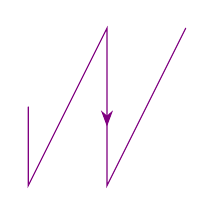
\begin{tikzpicture}[
    ->-/.style = {decoration={markings,
                    mark=at position .6 with {\arrow{Stealth[scale=1.2]}},},
                    postaction={decorate},cap=round}]
    \draw[->-,violet] (0,0) to ++(down:1) to ++(1,2) -- ++(down:2) -- ++(1,2);
\end{tikzpicture}
\end{document}

